\documentclass[11pt,oneside]{article}

\usepackage[letterpaper,margin=0.82in]{geometry}
\usepackage[T1]{fontenc}
\usepackage[utf8]{inputenc}
\usepackage{lmodern}
\usepackage{microtype}
\usepackage{amsmath,amssymb,amsthm,mathtools}
\usepackage{booktabs}
\usepackage{array}
\usepackage{longtable}
\usepackage{enumitem}
\usepackage{xcolor}
\usepackage{hyperref}
\usepackage{fancyhdr}
\usepackage{titlesec}
\usepackage{tikz}
\usepackage{pgfplots}
\usepackage{caption}
\usepackage{float}

\usetikzlibrary{arrows.meta,positioning,shapes.geometric,fit,calc,patterns,decorations.pathreplacing}
\pgfplotsset{compat=1.18}

\definecolor{ink}{HTML}{12263A}
\definecolor{coal}{HTML}{242424}
\definecolor{muted}{HTML}{59656F}
\definecolor{paper}{HTML}{FAF8F0}
\definecolor{gold}{HTML}{F2A541}
\definecolor{teal}{HTML}{2B9C8F}
\definecolor{brick}{HTML}{B74F3A}
\definecolor{bluegray}{HTML}{496A81}
\definecolor{softgreen}{HTML}{DDEBDD}
\definecolor{softgold}{HTML}{FFF0C9}
\definecolor{softred}{HTML}{F7D6D2}
\definecolor{softblue}{HTML}{DCEAF2}

\hypersetup{
  colorlinks=false,
  pdfborder={0 0 0},
  pdftitle={Context-Aware Skyline Reduction for GPU-First Combinatorial Optimization},
  pdfauthor={Emily Montes},
  pdfsubject={Skyline reduction, exact frontiers, and GPU-first optimization},
  pdfkeywords={skyline, frontier, Pareto, GPU, combinatorial optimization, dominance}
}

\pagestyle{fancy}
\fancyhf{}
\lhead{\small Context-Aware Skyline Reduction}
\rhead{\small Emily Montes}
\cfoot{\thepage}
\renewcommand{\headrulewidth}{0.4pt}
\renewcommand{\footrulewidth}{0pt}

\titleformat{\section}
  {\Large\bfseries}
  {\thesection}{0.65em}{}
\titleformat{\subsection}
  {\large\bfseries}
  {\thesubsection}{0.65em}{}
\titleformat{\subsubsection}
  {\normalsize\bfseries}
  {\thesubsubsection}{0.65em}{}

\setlist[itemize]{leftmargin=1.15em,itemsep=0.25em,topsep=0.35em}
\setlist[enumerate]{leftmargin=1.35em,itemsep=0.25em,topsep=0.35em}
\renewcommand{\arraystretch}{1.2}

\theoremstyle{definition}
\newtheorem{definition}{Definition}[section]
\newtheorem{assumption}{Assumption}[section]
\newtheorem{invariant}{Invariant}[section]
\newtheorem{theorem}{Theorem}[section]
\newtheorem{limitation}{Limitation}[section]

\newcommand{\Sky}{\operatorname{Sky}}
\newcommand{\Front}{\operatorname{Front}}
\newcommand{\ctx}{\mathcal{C}}
\newcommand{\cand}{\mathcal{X}}
\newcommand{\stats}{\Phi}
\newcommand{\score}{S}
\newcommand{\R}{\mathbb{R}}
\newcommand{\Policy}{\mathcal{P}}
\newcommand{\Cell}{\mathcal{K}}

\title{\vspace{-2.0em}\bfseries Context-Aware Skyline Reduction\\
\large for GPU-First Combinatorial Optimization}
\author{Emily Montes}
\date{May 10, 2026}

\begin{document}

\maketitle
\thispagestyle{plain}

\begin{abstract}

We study context-aware skyline reduction for GPU-first combinatorial optimization. The central problem is to reduce a large discrete candidate set before expensive device evaluation without discarding any candidate that can achieve the optimum under the intended objective. A conventional Pareto skyline can be unsafe when computed over raw feature vectors, because downstream scoring may depend on timing, budget, plateau, categorical compatibility, or objective-channel effects that are not represented in the raw vector. We therefore formulate skyline reduction over semantic cells: equivalence classes that preserve the information required for a dominance proof.

For a finite candidate set \(\cand\), a context family \(\ctx\), and a context-restricted score function \(\score_c\), we define a safe partial order \(\succeq_c\) only after the context \(c\) fixes the semantics of each feature. Under monotonicity in that context, the optimum over \(\cand_c\) equals the optimum over the non-dominated skyline \(\Sky_c(\cand_c)\). We also distinguish exact skylines from bounded frontiers, which are exact only relative to a declared policy objective unless additional dominance certificates exist. Finally, we describe how context-aware frontiers compose with exact GPU-facing inner solvers, how semantic cache identity affects correctness, and why broad raw-stat dominance should be treated as a visualization or initialization device rather than a pruning proof.

The result is a general pattern for optimization systems: partition first, prove local dominance second, evaluate retained frontiers third, and report objective channels without collapsing their semantics. This pattern favors small, explicit theorems over broad heuristics and is especially useful when GPU throughput is valuable but the candidate universe is too large to score indiscriminately.
\end{abstract}

\vspace{0.5em}
\noindent\textbf{Keywords:} combinatorial optimization; Pareto skyline; contextual dominance; GPU-first evaluation; exact frontiers; semantic cache correctness.

\section{Introduction}

High-dimensional combinatorial optimization often begins with the same practical question: how can a system search enough of the candidate universe to find excellent or exact results without evaluating an astronomical number of combinations? Hardware acceleration helps, but device throughput does not remove the need for mathematical selectivity. If a system evaluates dominated candidates faster, it still spends scarce compute on states that cannot change the answer.

Skyline reduction offers a principled alternative. A skyline is the set of candidates not dominated by any other candidate under a declared partial order. If one candidate is at least as good as another in every score-relevant dimension, then the weaker candidate can be discarded. This idea is standard in multi-objective optimization, databases, and Pareto frontier analysis. The subtlety is that real scoring systems rarely depend on raw vector components alone. They may include timing windows, caps, nonlinear lookup tables, discrete budget allocation, categorical compatibility, or multiple related objectives. These effects can make a broad raw-vector skyline unsound.

This manuscript argues for \emph{context-aware} skyline reduction. Rather than asking whether candidate \(y\) dominates candidate \(x\) globally, we ask whether \(y\) dominates \(x\) inside a context where the comparison is meaningful. The context may encode a timing cell, a surface identity, an objective channel, or another semantic equivalence class. Once the context fixes the interpretation of each coordinate, a local dominance theorem can be small, useful, and testable.

The approach is conservative. A local theorem that safely removes ten percent of a device payload may be more valuable than a global heuristic that removes ninety percent but occasionally loses the optimum. In optimization systems that publish best-known results or persist leaderboard-like outputs, an unsafe discard is not merely a performance bug. It is a correctness failure.

\subsection{Contributions}

This manuscript makes five general contributions:
\begin{itemize}
  \item A formal definition of context-aware skyline reduction for finite discrete optimization.
  \item A sufficiency theorem showing when a context skyline preserves the optimum.
  \item A warning theorem showing why cross-context raw dominance is not generally valid.
  \item A framework for distinguishing exact skylines from bounded policy frontiers.
  \item A model-card style risk analysis for GPU-first optimization systems that use semantic reduction before exact evaluation.
\end{itemize}

\section{Problem Setting}

Let \(\cand\) be a finite candidate universe. Each candidate \(x\in\cand\) is a compound decision state assembled from several discrete choice families:
\[
  \cand \subseteq
  \mathcal{A}_1 \times \mathcal{A}_2 \times \cdots \times \mathcal{A}_m
  \times \mathcal{T}
  \times \mathcal{V}.
\]
Here the \(\mathcal{A}_i\) represent abstract choice groups, \(\mathcal{T}\) represents timing or activation structure, and \(\mathcal{V}\) represents objective variants or evaluation modes. The score is a function:
\[
  \score : \cand \rightarrow \R.
\]
In practice, \(\score\) is rarely a simple linear function. It may be better represented as:
\[
  \score(x)
  =
  G\!\left(
    r(x),
    \tau(x),
    b(x),
    q(x),
    v(x)
  \right),
\]
where \(r(x)\) is a raw feature vector, \(\tau(x)\) is timing semantics, \(b(x)\) is budget state, \(q(x)\) is categorical compatibility, and \(v(x)\) is the active objective variant. These symbols are general abstractions.

\begin{definition}[Context]
A context \(c\in\ctx\) is a semantic equivalence class that fixes enough information for a dominance relation to be valid. It may fix timing behavior, objective channel, budget interpretation, categorical compatibility, or policy identity.
\end{definition}

\begin{definition}[Context-restricted candidate set]
For a context \(c\), \(\cand_c\subseteq\cand\) is the subset of candidates whose comparison semantics are fixed by \(c\).
\end{definition}

\begin{definition}[Context feature map]
A context feature map is a function
\[
  \stats_c : \cand_c \rightarrow \R^d
\]
whose coordinates are sufficient for safe comparison inside \(c\).
\end{definition}

The optimization goal for each context is:
\[
  x_c^* \in \arg\max_{x\in\cand_c} \score_c(x).
\]
A reduction is lossless when it preserves this optimum.

\section{Why Raw Skylines Are Not Enough}

A raw skyline is computed from a feature map \(r:\cand\rightarrow\R^d\). Candidate \(y\) raw-dominates candidate \(x\) if:
\[
  r_i(y) \ge r_i(x)\quad\forall i.
\]
This relation is safe only when score is monotone in \(r\) over the compared domain. The problem is hidden context. If score depends on \(h(x)\) as well as \(r(x)\), then raw dominance gives:
\[
  r(y)\ge r(x),
\]
but does not imply:
\[
  G(r(y),h(y))\ge G(r(x),h(x)).
\]

\subsection{Common sources of unsoundness}
\begin{itemize}
  \item \textbf{Timing dependence.} A coordinate can be valuable in one timing region and irrelevant in another.
  \item \textbf{Plateaus.} More raw value can map to the same effective value after discretization or lookup.
  \item \textbf{Caps.} Once a cap binds, extra raw value may not improve the score.
  \item \textbf{Budget coupling.} A stronger raw candidate may consume a scarce resource needed elsewhere.
  \item \textbf{Categorical compatibility.} Numeric totals can hide whether the value belongs to the active category.
  \item \textbf{Objective variants.} The candidate that optimizes one objective channel may be suboptimal for another.
\end{itemize}

\begin{figure}[H]
\centering
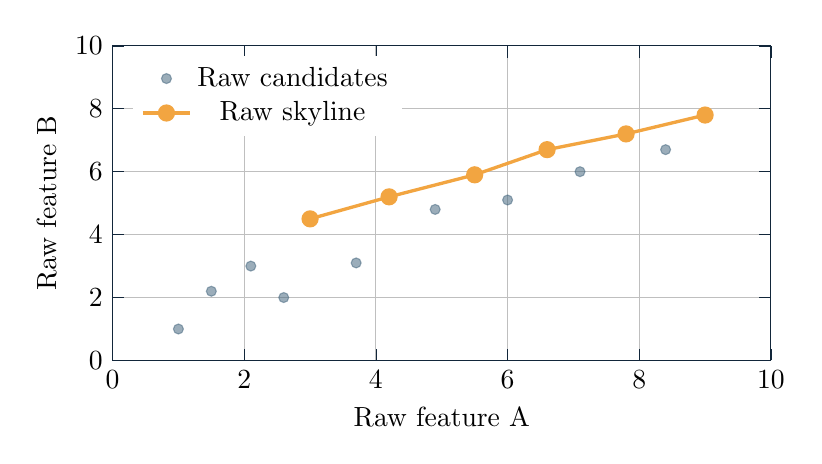
\begin{tikzpicture}
\begin{axis}[
  width=0.82\textwidth,
  height=0.46\textwidth,
  xlabel={Raw feature A},
  ylabel={Raw feature B},
  xmin=0,xmax=10,
  ymin=0,ymax=10,
  grid=major,
  axis line style={draw=ink},
  tick style={draw=ink},
  legend style={draw=none,fill=white,at={(0.03,0.97)},anchor=north west},
]
\addplot[only marks,mark=*,mark size=1.8pt,color=bluegray,opacity=0.55] coordinates {
  (1,1) (1.5,2.2) (2.1,3.0) (2.6,2.0) (3.0,4.5)
  (3.7,3.1) (4.2,5.2) (4.9,4.8) (5.5,5.9) (6.0,5.1)
  (6.6,6.7) (7.1,6.0) (7.8,7.2) (8.4,6.7) (9.0,7.8)
};
\addplot[very thick,color=gold,mark=*,mark size=2.5pt] coordinates {
  (3.0,4.5) (4.2,5.2) (5.5,5.9) (6.6,6.7) (7.8,7.2) (9.0,7.8)
};
\addlegendentry{Raw candidates}
\addlegendentry{Raw skyline}
\end{axis}
\end{tikzpicture}
\caption{Synthetic two-dimensional example of a raw skyline that is mathematically correct for raw vectors while still being insufficient for downstream score semantics.}
\end{figure}

\section{Context-Aware Dominance}

\begin{definition}[Contextual dominance]
For \(x,y\in\cand_c\), define
\[
  y\succeq_c x
  \quad\Longleftrightarrow\quad
  \stats_c(y)_i\ge \stats_c(x)_i
  \quad \forall i\in\{1,\ldots,d\}.
\]
If at least one inequality is strict, or if a certified tie-break relation holds, then \(y\) strictly dominates \(x\) in context \(c\).
\end{definition}

\begin{definition}[Context skyline]
The context skyline is
\[
  \Sky_c(\cand_c)
  =
  \left\{
    x\in\cand_c:
    \nexists y\in\cand_c
    \text{ such that } y\succeq_c x
    \text{ and } y\not\equiv_c x
  \right\}.
\]
The equivalence relation \(\equiv_c\) captures score-preserving ties that may still differ operationally.
\end{definition}

\begin{assumption}[Context monotonicity]
For a fixed context \(c\), score is monotone under contextual dominance:
\[
  y\succeq_c x
  \quad\Longrightarrow\quad
  \score_c(y)\ge\score_c(x).
\]
\end{assumption}

\begin{theorem}[Skyline sufficiency]
If context monotonicity holds for \(c\), then
\[
  \max_{x\in\cand_c}\score_c(x)
  =
  \max_{x\in\Sky_c(\cand_c)}\score_c(x).
\]
\end{theorem}

\begin{proof}
Every candidate is either non-dominated or dominated by another candidate. If \(x\) is dominated by \(y\), monotonicity gives \(\score_c(y)\ge\score_c(x)\). Because \(\cand_c\) is finite, repeated replacement by a dominating candidate terminates at a non-dominated representative with score at least as high as the original. Therefore the best discarded candidate cannot exceed the best skyline candidate.
\end{proof}

\subsection{Interpretation}
The theorem is simple because the hard work is in the context definition. The comparison must include every semantic dimension that can affect score ordering. If a dimension is omitted, the theorem may no longer apply.

\section{Timing Cells and Semantic Cells}

A semantic cell is the region in which feature comparisons have stable meaning. Timing cells are a common example. Two candidates may have the same raw values but place those values into different score-relevant intervals. Conversely, two candidates may have different raw values but collapse to the same effective behavior inside a timing cell.

\begin{definition}[Semantic cell]
A semantic cell \(k\in\Cell\) is a subset \(\cand_k\subseteq\cand\) such that all candidates in \(\cand_k\) share the semantics required by a chosen dominance relation.
\end{definition}

\begin{theorem}[No cross-cell dominance without proof]
Let \(k_1\) and \(k_2\) be semantic cells. A dominance relation proven in \(k_1\) is not valid for comparisons with \(k_2\) unless an additional theorem proves invariance across both cells.
\end{theorem}

\begin{proof}
A dominance proof in \(k_1\) establishes monotonicity under the semantics fixed by \(k_1\). If a candidate lies in \(k_2\), its timing, budget, categorical, or objective semantics may differ. The score function may therefore assign different marginal value to the same coordinate. The implication required for dominance is not established across cells.
\end{proof}

\subsection{A useful motto}
\[
  \boxed{\text{No declared cell, no dominance certificate.}}
\]
This rule prevents attractive but unsafe reductions from being treated as exact.

\begin{figure}[H]
\centering
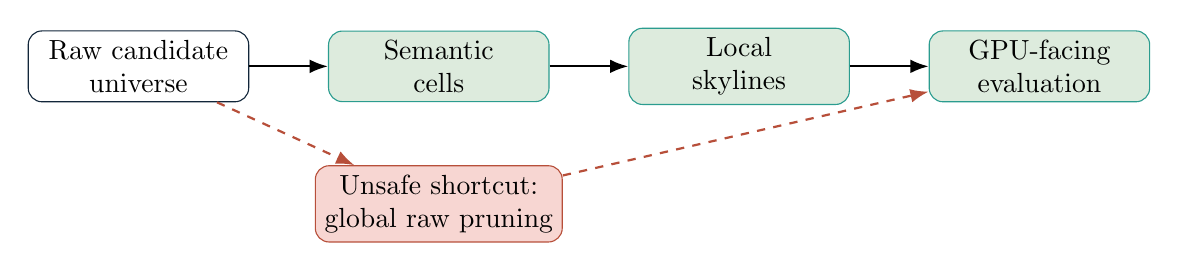
\begin{tikzpicture}[node distance=1.0cm,>=Latex]
  \tikzstyle{box}=[draw=ink,rounded corners=5pt,fill=white,minimum width=2.8cm,minimum height=0.72cm,align=center]
  \tikzstyle{safe}=[draw=teal,rounded corners=5pt,fill=softgreen,minimum width=2.8cm,minimum height=0.72cm,align=center]
  \tikzstyle{warn}=[draw=brick,rounded corners=5pt,fill=softred,minimum width=2.8cm,minimum height=0.72cm,align=center]
  \node[box] (raw) {Raw candidate\\universe};
  \node[safe,right=of raw] (cell) {Semantic\\cells};
  \node[safe,right=of cell] (sky) {Local\\skylines};
  \node[safe,right=of sky] (gpu) {GPU-facing\\evaluation};
  \node[warn,below=0.8cm of cell] (bad) {Unsafe shortcut:\\global raw pruning};
  \draw[->,thick] (raw) -- (cell);
  \draw[->,thick] (cell) -- (sky);
  \draw[->,thick] (sky) -- (gpu);
  \draw[->,thick,dashed,draw=brick] (raw) -- (bad);
  \draw[->,thick,dashed,draw=brick] (bad) -- (gpu);
\end{tikzpicture}
\caption{Context-aware reduction compares candidates only after semantic partitioning.}
\end{figure}

\section{Exact Evaluation After Reduction}

A skyline is valuable because it can make exact evaluation feasible. The reduction and evaluation stages compose if each stage preserves its own invariant.

\begin{assumption}[Lossless retained set]
A retained set \(R_c\subseteq\cand_c\) is lossless when
\[
  \max_{x\in R_c}\score_c(x)
  =
  \max_{x\in\cand_c}\score_c(x).
\]
\end{assumption}

\begin{assumption}[Exact evaluator]
An evaluator \(E\) is exact over \(R_c\) when
\[
  E(R_c)=\max_{x\in R_c}\score_c(x).
\]
\end{assumption}

\begin{theorem}[Compositional exactness]
If \(R_c\) is lossless and \(E\) is exact over \(R_c\), then
\[
  E(R_c)=\max_{x\in\cand_c}\score_c(x).
\]
\end{theorem}

\begin{proof}
Substitute the retained-set equality into the evaluator equality.
\end{proof}

\subsection{Engineering interpretation}
The exactness claim is modular. A failure can be localized to one of three boundaries:
\begin{itemize}
  \item the semantic partition is too coarse,
  \item the dominance relation discards a possible optimum,
  \item the evaluator is not exact over the retained set.
\end{itemize}

\subsection{GPU-first motivation}
When exact evaluation is expensive, it should run where the system is designed to run heavy scoring. Context-aware reduction should prepare smaller, cleaner device work rather than replacing the device path with host-side production scoring.

\section{Bounded Frontiers}

Some contexts have large skylines. A bounded frontier keeps at most \(k\) representatives per cell under a declared policy. This is useful but changes the exactness claim.

\begin{definition}[Policy-bounded frontier]
For policy \(\Policy_c\) and width \(k\), define
\[
  \Front_{c,k}(\cand_c)
  =
  \operatorname{TopK}_{\Policy_c}\!\left(\Sky_c(\cand_c),k\right).
\]
\end{definition}

\begin{theorem}[Bounded exactness is policy-relative]
A bounded frontier is exact for the declared policy objective if the downstream evaluator optimizes that same policy over the retained set. It is not necessarily exact for a different objective.
\end{theorem}

\begin{proof}
If \(|\Sky_c(\cand_c)|>k\), bounded retention discards non-dominated points. Since those points are not dominated under \(\succeq_c\), discarding them requires an additional ranking policy. A different objective may prefer a discarded point unless a separate dominance certificate rules it out.
\end{proof}

\subsection{Honest language}
The phrase ``exact frontier'' should always be accompanied by scope:
\begin{itemize}
  \item exact for which context,
  \item exact for which policy,
  \item exact under which width,
  \item exact under which score semantics.
\end{itemize}

\begin{figure}[H]
\centering
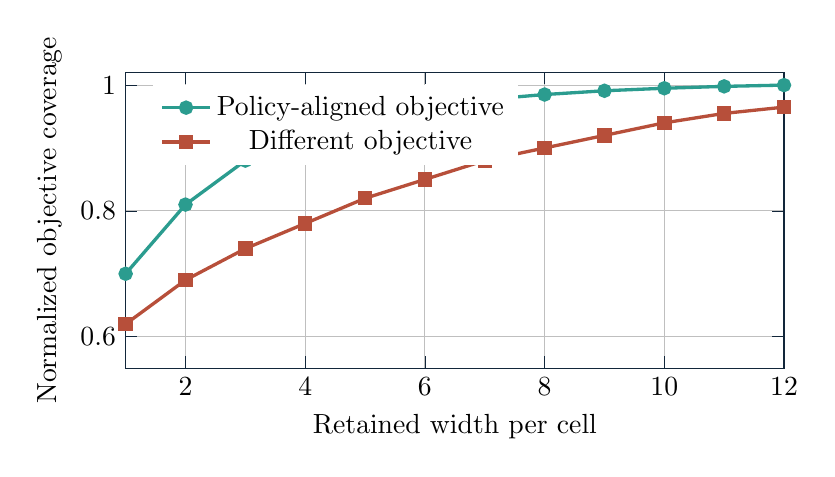
\begin{tikzpicture}
\begin{axis}[
  width=0.82\textwidth,
  height=0.44\textwidth,
  xlabel={Retained width per cell},
  ylabel={Normalized objective coverage},
  xmin=1,xmax=12,
  ymin=0.55,ymax=1.02,
  grid=major,
  axis line style={draw=ink},
  tick style={draw=ink},
  legend style={draw=none,fill=white,at={(0.04,0.96)},anchor=north west},
]
\addplot[very thick,color=teal,mark=*] coordinates {
  (1,0.70) (2,0.81) (3,0.88) (4,0.92) (5,0.95) (6,0.965)
  (7,0.977) (8,0.985) (9,0.991) (10,0.995) (11,0.998) (12,1.0)
};
\addplot[very thick,color=brick,mark=square*] coordinates {
  (1,0.62) (2,0.69) (3,0.74) (4,0.78) (5,0.82) (6,0.85)
  (7,0.88) (8,0.90) (9,0.92) (10,0.94) (11,0.955) (12,0.965)
};
\addlegendentry{Policy-aligned objective}
\addlegendentry{Different objective}
\end{axis}
\end{tikzpicture}
\caption{Synthetic bounded-frontier behavior. A width that is nearly complete for one policy may be insufficient for another.}
\end{figure}

\section{Algorithmic Pattern}

\begin{longtable}{>{\raggedright\arraybackslash}p{0.12\textwidth}>{\raggedright\arraybackslash}p{0.78\textwidth}}
\toprule
\textbf{Step} & \textbf{Action} \\
\midrule
1 & Partition the candidate set into semantic cells using a deterministic context builder. \\
2 & For each cell, expose only the feature map known to be sufficient for that cell's dominance proof. \\
3 & Maintain a local skyline by removing candidates dominated under the cell relation. \\
4 & Optionally apply a bounded policy frontier, while preserving the policy identity in the exactness claim. \\
5 & Send retained frontiers to the accelerator-facing evaluator. \\
6 & Report objective channels independently and retain enough audit metadata to explain the reduction. \\
\bottomrule
\end{longtable}

\subsection{Important implementation-independent requirements}
\begin{itemize}
  \item The context builder must be deterministic for the same semantic inputs.
  \item The dominance relation must not inspect omitted hidden context.
  \item The retained frontier must preserve enough metadata for audit and reporting.
  \item The reduction should not become a production bottleneck before device submission.
\end{itemize}

\subsection{Complexity intuition}
If \(n_c=|\cand_c|\) and \(f_c=|\Sky_c(\cand_c)|\), a naive skyline construction may be \(O(n_c f_c d)\) per cell. More sophisticated data structures can improve this for certain dimensions and distributions, but the essential tradeoff remains: the reduction is worthwhile when it is cheaper than evaluating candidates that cannot win.

\section{Device Scheduling Considerations}

The skyline idea can fail operationally even when it is mathematically safe. If a host-side reducer performs expensive work before any device work is submitted, the accelerator can become idle or bursty. A GPU-first optimizer should treat device saturation as an architectural invariant, not an afterthought.

\begin{invariant}[GPU-first evaluation]
Heavy production scoring should remain on the accelerator-facing path. Host-side reductions should prepare smaller and more meaningful device work, not replace the production evaluator with a hidden serial bottleneck.
\end{invariant}

\subsection{Safe placement}
A reduction is most attractive when it is:
\begin{itemize}
  \item cheap enough to run before packing device work,
  \item reusable across multiple device batches,
  \item or computed after a first device-visible surface exists.
\end{itemize}

\subsection{Risky placement}
A reduction is risky when it:
\begin{itemize}
  \item scans many candidate pairs before first device submission,
  \item duplicates work already performed by the exact evaluator,
  \item serializes an otherwise parallel pipeline,
  \item or introduces a host-only production scoring path.
\end{itemize}

\begin{figure}[H]
\centering
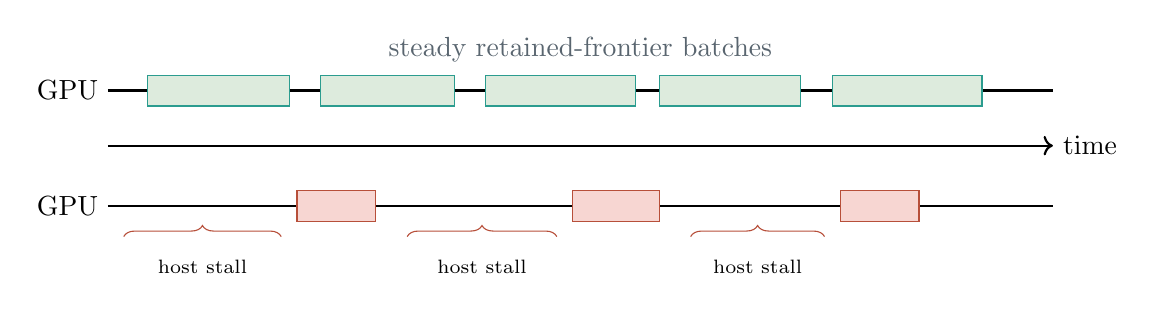
\begin{tikzpicture}[x=1cm,y=0.7cm]
  \draw[->,thick] (0,0) -- (12,0) node[right] {time};
  \draw[thick] (0,1) -- (12,1);
  \node[left] at (0,1) {GPU};
  \foreach \x/\w in {0.5/1.8,2.7/1.7,4.8/1.9,7.0/1.8,9.2/1.9} {
    \draw[fill=softgreen,draw=teal] (\x,0.72) rectangle +(\w,0.56);
  }
  \node[align=center,color=muted] at (6,1.75) {steady retained-frontier batches};
  \draw[thick] (0,-1.1) -- (12,-1.1);
  \node[left] at (0,-1.1) {GPU};
  \foreach \x/\w in {2.4/1.0,5.9/1.1,9.3/1.0} {
    \draw[fill=softred,draw=brick] (\x,-1.38) rectangle +(\w,0.56);
  }
  \foreach \x/\w in {0.2/2.0,3.8/1.9,7.4/1.7} {
    \draw[decorate,decoration={brace,amplitude=4pt},draw=brick] (\x,-1.65) -- +(\w,0) node[midway,below=5pt,font=\scriptsize] {host stall};
  }
\end{tikzpicture}
\caption{Conceptual device utilization. Safe reductions keep work flowing; poorly placed reductions can create bursty accelerator use.}
\end{figure}

\section{Semantic Cache Correctness}

Frontier construction may be cached. A cache is correct only when its key includes all semantic inputs that can change the frontier.

\begin{definition}[Complete semantic key]
A cache key \(K\) is complete for builder \(B\) if
\[
  K(a)=K(b)
  \quad\Longrightarrow\quad
  B(a)=B(b).
\]
\end{definition}

\begin{theorem}[Cache soundness]
If \(K\) is complete and a cached value was generated by the same builder policy, then loading the cached frontier is equivalent to rebuilding it.
\end{theorem}

\begin{proof}
By completeness, equal keys imply equal builder outputs. If the stored value is the builder output for that key and policy, the loaded value equals the rebuilt value.
\end{proof}

\subsection{Semantic key components}
The key decomposes as:
\[
  K =
  \text{input identity}
  + \text{context identity}
  + \text{feature-map identity}
  + \text{policy identity}
  + \text{score-semantics identity}.
\]

\subsection{Why cache identity is correctness, not speed}
If a frontier policy changes but the cache key does not, the system may silently reuse an obsolete retained set. That can preserve an old theorem while the evaluator assumes a new one. Cache identity therefore belongs in the correctness model.

\section{Multiple Objective Channels}

Many optimizers expose related but distinct objective channels. For example, one channel may represent a base score and another may represent a constrained variant. The exact names do not matter. What matters is that the maxima may differ.

\begin{invariant}[Separated objective channels]
For objectives \(\score_a\) and \(\score_b\), report and persist:
\[
  \operatorname{Best}_a=\max_x\score_a(x),
  \qquad
  \operatorname{Best}_b=\max_x\score_b(x),
\]
without assuming the same candidate attains both maxima.
\end{invariant}

\begin{theorem}[No silent channel merge]
If there exist candidates \(x,y\) such that
\[
  \score_a(x)>\score_a(y)
  \quad\text{and}\quad
  \score_b(y)>\score_b(x),
\]
then using one channel's winner for both channels is unsound.
\end{theorem}

\begin{proof}
The inequalities show that the channels prefer different candidates. A single reported winner cannot be correct for both objectives unless additional transformation logic is applied and proven.
\end{proof}

\subsection{Relevance to skyline reduction}
A dominance relation may be valid for one objective channel and invalid for another. Therefore objective identity is part of context. A retained frontier for one channel should not automatically be reused as the exact frontier for another.

\section{Conceptual Evaluation Framework}

We use synthetic normalized examples to make the evaluation targets explicit. The framework defines what an implementation should measure: preservation of optima, retained frontier width, accelerator scheduling behavior, cache validity, and objective-channel separation.

\subsection{Evaluation questions}
\begin{itemize}
  \item Does contextual skyline reduction preserve the optimum on adversarial small cases?
  \item Does the retained frontier shrink enough to justify construction cost?
  \item Does the reducer avoid blocking the accelerator-facing path?
  \item Do semantic cache keys invalidate when policy or score semantics change?
  \item Are objective channels evaluated and reported independently?
\end{itemize}

\subsection{Recommended proof gates}
\begin{longtable}{>{\raggedright\arraybackslash}p{0.24\textwidth}>{\raggedright\arraybackslash}p{0.37\textwidth}>{\raggedright\arraybackslash}p{0.29\textwidth}}
\toprule
\textbf{Gate} & \textbf{Question} & \textbf{Pass condition} \\
\midrule
Dominance gate & Is the partial order valid in this context? & Every discarded candidate is dominated under all score-relevant coordinates. \\
Counterexample gate & Does a broader theorem fail? & Unsafe generalizations are blocked or documented as non-production claims. \\
Exactness gate & Does the evaluator optimize over the retained set? & Exact evaluator matches a trusted narrow reference. \\
Cache gate & Does key identity include semantic inputs? & Policy changes cannot reuse stale frontiers. \\
Device gate & Does reduction preserve accelerator flow? & Heavy scoring remains on the accelerator-facing path. \\
Output gate & Are objective channels separate? & Distinct objectives retain distinct winners when necessary. \\
\bottomrule
\end{longtable}

\section{Conceptual Reduction Curves}

\begin{figure}[H]
\centering
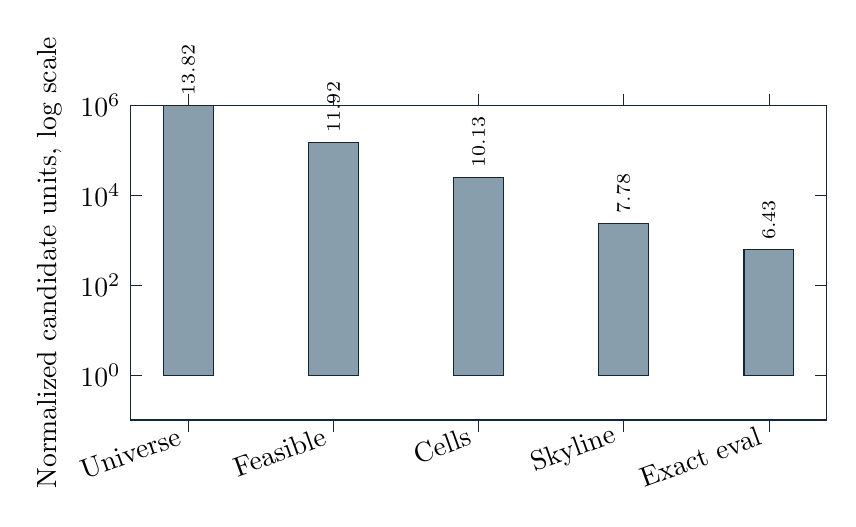
\begin{tikzpicture}
\begin{axis}[
  ybar,
  width=0.86\textwidth,
  height=0.46\textwidth,
  symbolic x coords={Universe,Feasible,Cells,Skyline,Exact eval},
  xtick=data,
  x tick label style={rotate=20,anchor=east},
  ymin=0.1,
  ymax=1000000,
  ymode=log,
  ylabel={Normalized candidate units, log scale},
  nodes near coords,
  every node near coord/.append style={font=\scriptsize,rotate=90,anchor=west},
  bar width=18pt,
  axis line style={draw=ink},
  tick style={draw=ink},
]
\addplot[fill=bluegray!65,draw=ink] coordinates {
  (Universe,1000000)
  (Feasible,150000)
  (Cells,25000)
  (Skyline,2400)
  (Exact eval,620)
};
\end{axis}
\end{tikzpicture}
\caption{Synthetic reduction funnel for a context-aware skyline pipeline.}
\end{figure}

\subsection{Interpretation}
The useful question is not simply how many candidates were removed. It is whether the removed candidates were proved irrelevant in context. A smaller frontier is valuable only if it preserves the optimum claimed by the system.

\begin{figure}[H]
\centering
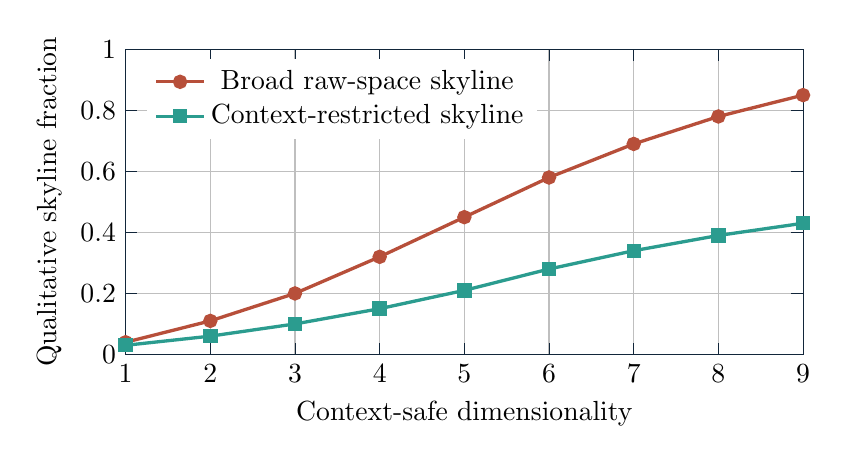
\begin{tikzpicture}
\begin{axis}[
  width=0.84\textwidth,
  height=0.45\textwidth,
  xlabel={Context-safe dimensionality},
  ylabel={Qualitative skyline fraction},
  xmin=1,xmax=9,
  ymin=0,ymax=1,
  grid=major,
  axis line style={draw=ink},
  tick style={draw=ink},
  legend style={draw=none,fill=white,at={(0.03,0.97)},anchor=north west},
]
\addplot[very thick,color=brick,mark=*] coordinates {
  (1,0.04) (2,0.11) (3,0.20) (4,0.32) (5,0.45) (6,0.58) (7,0.69) (8,0.78) (9,0.85)
};
\addplot[very thick,color=teal,mark=square*] coordinates {
  (1,0.03) (2,0.06) (3,0.10) (4,0.15) (5,0.21) (6,0.28) (7,0.34) (8,0.39) (9,0.43)
};
\addlegendentry{Broad raw-space skyline}
\addlegendentry{Context-restricted skyline}
\end{axis}
\end{tikzpicture}
\caption{Conceptual antichain risk. Context restriction can reduce skyline width by avoiding irrelevant comparison dimensions.}
\end{figure}

\section{Risk Register}

\begin{longtable}{>{\raggedright\arraybackslash}p{0.24\textwidth}>{\raggedright\arraybackslash}p{0.30\textwidth}>{\raggedright\arraybackslash}p{0.32\textwidth}}
\toprule
\textbf{Risk} & \textbf{Failure mode} & \textbf{Mitigation} \\
\midrule
Over-broad dominance & Drops a true optimum because hidden context changes score meaning. & Require declared cells and adversarial counterexamples. \\
Stale frontier cache & Reuses old retained sets after policy changes. & Include semantic policy identity in the cache key. \\
Host-side bottleneck & Safe reduction delays accelerator work. & Keep pre-device reductions cheap or move them later. \\
Bounded-frontier ambiguity & Describes a policy frontier as globally exact. & State objective, width, and context for every exactness claim. \\
Objective-channel collapse & Reports one channel's winner as another's. & Evaluate and report distinct objectives independently. \\
Metric theatre & Reports speedup without correctness evidence. & Pair performance claims with invariant-targeted proof gates. \\
\bottomrule
\end{longtable}

\begin{figure}[H]
\centering
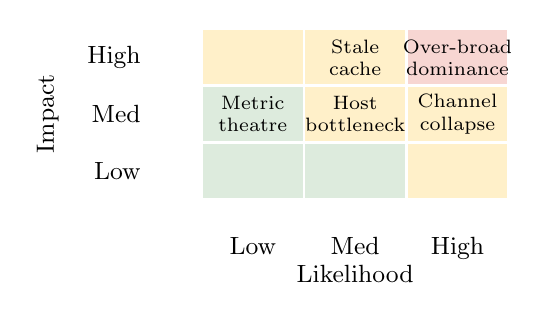
\begin{tikzpicture}[x=1.3cm,y=0.72cm]
  \foreach \x/\label in {1/Low,2/Med,3/High} {
    \node[anchor=north] at (\x,0) {\small \label};
  }
  \foreach \y/\label in {1/Low,2/Med,3/High} {
    \node[anchor=east] at (0,\y) {\small \label};
  }
  \node[anchor=north] at (2,-0.5) {\small Likelihood};
  \node[rotate=90,anchor=south] at (-0.8,2) {\small Impact};
  \foreach \x in {1,2,3} {
    \foreach \y in {1,2,3} {
      \pgfmathtruncatemacro{\scorecell}{\x+\y}
      \ifnum\scorecell<4
        \def\cellcolor{softgreen}
      \else
        \ifnum\scorecell<6
          \def\cellcolor{softgold}
        \else
          \def\cellcolor{softred}
        \fi
      \fi
      \draw[fill=\cellcolor,draw=white,line width=1pt] (\x-0.5,\y-0.5) rectangle (\x+0.5,\y+0.5);
    }
  }
  \node[align=center,font=\scriptsize] at (3,3) {Over-broad\\dominance};
  \node[align=center,font=\scriptsize] at (2,3) {Stale\\cache};
  \node[align=center,font=\scriptsize] at (3,2) {Channel\\collapse};
  \node[align=center,font=\scriptsize] at (2,2) {Host\\bottleneck};
  \node[align=center,font=\scriptsize] at (1,2) {Metric\\theatre};
\end{tikzpicture}
\caption{Qualitative risk matrix for context-aware skyline systems.}
\end{figure}

\section{Related Mathematical Ideas}

\subsection{Pareto optimality}
The skyline is a finite-set version of Pareto optimality. It keeps points for which no other point is at least as good in all dimensions and strictly better in at least one. The contribution here is not the skyline itself, but the insistence that the dimensions must be context-safe.

\subsection{Branch and bound}
Exact inner evaluation often resembles branch and bound: compute upper bounds, prune impossible branches, and search the retained feasible region. Context-aware skylines complement this by shrinking the input before exact search begins.

\subsection{Dynamic programming over small surfaces}
When a retained frontier is small and structured, dynamic programming can become feasible. The frontier serves as a compact state surface over which exact recurrence or bounded recurrence can run.

\subsection{Database skylines}
Skyline queries in databases often assume that dimensions directly represent user preference. Optimization scoring may violate that assumption because preferences are mediated by hidden semantics. This is why semantic cells are necessary.

\section{Discussion}

The main practical lesson is that skyline reduction is not a single algorithmic switch. It is a discipline for making invalid comparisons impossible. The strongest versions of this discipline share four habits.

\subsection{Name the context}
Every dominance claim should begin with the context that makes it true. If the context cannot be named, the claim is not ready to prune candidates.

\subsection{Prefer exact local theorems}
A narrow theorem that applies to a common cell can be more useful than a broad theorem that fails on edge cases. Local exactness is composable. Global overclaiming is fragile.

\subsection{Keep the accelerator busy}
Mathematical reduction should serve the compute architecture. If reduction becomes a serial gate before device work, the system may lose the practical benefit of smaller frontiers.

\subsection{Separate objectives}
If a system has multiple score channels, each channel needs its own exactness story. A candidate can be best for one channel and not another.

\section{Limitations}

\begin{limitation}[No universal raw dominance]
Raw-vector dominance is not universally safe for nonlinear, context-dependent scoring systems.
\end{limitation}

\begin{limitation}[Large antichains]
In high-dimensional spaces, many candidates may be mutually non-dominated, limiting compression.
\end{limitation}

\begin{limitation}[Bounded frontier scope]
A bounded frontier can be exact for a declared policy but not automatically exact for all objectives.
\end{limitation}

\begin{limitation}[Empirical dependence]
Measured curves depend on the candidate distribution, semantic partition, accelerator, batching strategy, and exact evaluator.
\end{limitation}

\begin{limitation}[Implementation dependence]
Actual performance depends on data distribution, device architecture, batching strategy, memory layout, and cache behavior.
\end{limitation}

\section{Conclusion}

Context-aware skyline reduction provides a principled pattern for reducing large candidate sets before GPU-first exact evaluation. Its central rule is simple: dominance is safe only in the semantic context where score meaning is preserved. This rule blocks broad but unsafe raw-stat pruning while enabling local, exact, and testable reductions.

The pattern is especially attractive for optimization systems with nonlinear scoring, timing effects, budget constraints, categorical compatibility, and multiple objective channels. It converts the performance problem from ``score everything faster'' into ``prove what can still matter, then score that exactly.'' When combined with semantic cache identity and accelerator-aware scheduling, context-aware skylines can reduce work without weakening correctness claims.

The resulting research posture is conservative but powerful. It treats exactness as a scoped statement, bounded frontiers as policy-relative objects, and negative results as valuable guardrails. In systems where a single discarded optimum is unacceptable, that discipline is not optional. It is the difference between a fast heuristic and a reliable optimizer.

\section*{Appendix A: Glossary}
\addcontentsline{toc}{section}{Appendix A: Glossary}

\begin{longtable}{>{\raggedright\arraybackslash}p{0.28\textwidth}>{\raggedright\arraybackslash}p{0.62\textwidth}}
\toprule
\textbf{Term} & \textbf{Meaning} \\
\midrule
Candidate & A possible decision state considered by an optimizer. \\
Context & A semantic environment that makes candidate comparison valid. \\
Cell & A group of candidates sharing enough semantics for safe reduction. \\
Dominance & A partial order where one candidate is at least as good in every relevant dimension. \\
Skyline & The non-dominated subset under a declared dominance relation. \\
Frontier & The retained candidate surface after skyline or policy reduction. \\
Bounded frontier & A frontier capped by a declared policy, exact only under that policy's scope. \\
Exact evaluator & A scoring stage that finds the optimum over its retained input set. \\
GPU-first & Heavy production scoring is designed around accelerator execution. \\
Objective channel & A distinct score surface with its own optimum and reporting semantics. \\
Proof gate & A test or argument that blocks unsafe reductions from being treated as exact. \\
Antichain & A set where no candidate dominates another. \\
\bottomrule
\end{longtable}

\section*{Appendix B: Mathematical Summary}
\addcontentsline{toc}{section}{Appendix B: Mathematical Summary}

Let \(\cand\) be finite and let \(\ctx\) be a set of semantic contexts. For each \(c\in\ctx\), define \(\cand_c\subseteq\cand\), a feature map \(\stats_c:\cand_c\rightarrow\R^d\), and a score function \(\score_c:\cand_c\rightarrow\R\). Define:
\[
  y\succeq_c x
  \iff
  \stats_c(y)_i\ge\stats_c(x)_i
  \quad\forall i.
\]
If
\[
  y\succeq_c x\Rightarrow\score_c(y)\ge\score_c(x),
\]
then
\[
  \max_{x\in\cand_c}\score_c(x)
  =
  \max_{x\in\Sky_c(\cand_c)}\score_c(x).
\]
For a bounded policy frontier:
\[
  \Front_{c,k}(\cand_c)
  =
  \operatorname{TopK}_{\Policy_c}\left(\Sky_c(\cand_c),k\right),
\]
exactness is scoped to \(\Policy_c\) unless another dominance theorem proves discarded skyline points irrelevant for other objectives.

The safest general pattern is:
\[
  \boxed{
  \text{partition into contexts}
  \rightarrow
  \text{prove local dominance}
  \rightarrow
  \text{retain skyline/frontier}
  \rightarrow
  \text{evaluate exactly}
  }
\]

\end{document}

